\section{Algoritmo de traducci\'on de experimentos}

Un programa almacenable y ejecutable en el PP2 es una secuencia de 
instrucciones \(I_{1} ... I_{N}\) con \(1 \leq N \leq 512 \).
\\
Donde las instrucciones disponibles son:

\begin{itemize}
    \item $Continue$
    \item $Loop$
    \item $Retl$
    \item $End$
\end{itemize}

\noindent
No todos los programas escritos con estas instrucciones son admitidos 
como v\'alidos para el PP2, por esto tenemos las siguientes reglas:

\begin{itemize}
\item Regla 1: la instrucci\'on $End$ siempre es la \'ultima.
\item Regla 2: la instrucci\'on $End$ aparece s\'olo una vez.
\item Regla 3: la instrucci\'on $End$ siempre est\'a presente.
\item Regla 4: un bucle siempre inicia con instrucci\'on $Loop$ y finaliza con $Retl$.
\item Regla 5: puede haber hasta 3 instrucciones $Loop$ anidados en un $Loop$.
\item Regla 6: la longitud del programa no puede ser mayor a 512 instrucciones.
\end{itemize}

\begin{figure}[!htb].
    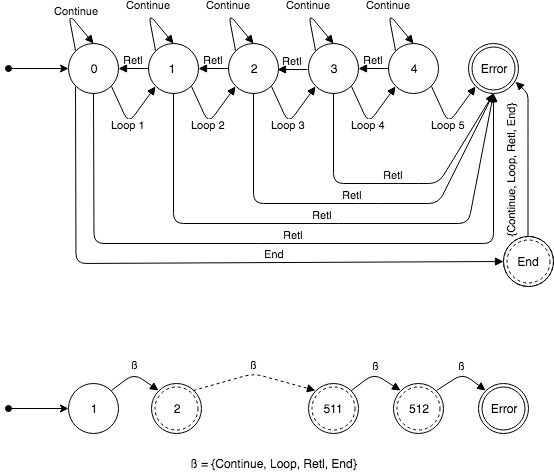
\includegraphics[width=\linewidth]{../figures/d12.jpg}
    \caption{Los programas aceptados por el PP2.}
    \label{fig:d12}
\end{figure}
 
\newpage

\begin{algorithm}
    \caption{Algoritmo de traducci\'on base}\label{euclid}
    \begin{algorithmic}[1]
    \Procedure{Translate}{P, L=0, S=[]}
    \State \Assert{$len(S) \leq 512$}
    \State $ins \gets pop(P)$

    \If {$ins = Continue$}
    \State S.append(ins)
    \State $Translate(P, L, S)$
    \EndIf

    \If {$ins = Retl$}
        \If {$L > 0$}
            \State $S.append(\textit{ins})$
            \State $L \gets L-1$
            \State $Translate(P, L, S)$
        \Else
            \State \Return $error$
        \EndIf
    \EndIf
    
    \If {$ins = Loop$}
        \If {$L < 4$}
            \State $S.append(\textit{ins})$
            \State $L \gets L+1$
            \State $Translate(P, L, S)$
        \Else
            \State \Return $error$
        \EndIf
    \EndIf

    \If {$ins = End $}
        \If {$len(P) = 0 \land L = 0$}
            \State $S.append(\textit{ins})$
        \Else
            \State \Return $error$
        \EndIf
    \EndIf

    \State \Assert{$ 1 \leq len(S) \leq 512$}
    \State \Assert{$ last(S) = End$}
    \State \Return $S$
    \EndProcedure
    \end{algorithmic}
    \end{algorithm}
    
% traslate(P, L, S)

%     ins = next(P)

%     if ins = Continue:
%         S.append(ins)

%     if ins = Retl:
%         if(L!=0):
%             S.append(ins)
%             L--
%         else:
%             ret Error

%     if ins = Loop:
%         if(L<4):
%             S.append(ins)
%             L++
%         else:
%             ret Error
    
%     ret S

El algoritmo desapila instrucciones de $P$ y seg\'un el tipo se valida de manera distinta.
La variable $L$ cuenta el n\'umero de Loops abiertos al momento, si es mayor a 4 finaliza en error
caso contrario se agrega la instrucci\'on a la secuencia $S$ y se aplica recursi\'on.
El \'unico caso donde no hay recursividad es cuando la instrucci\'on desapilada es $End$
donde si hay mas intrucciones por desapilar de $P$ \'o el contador $L$ es no esta en 0 termina en error
caso contrario se agrega $End$ a la secuencia $S$ y se valida al final que $S$ contenga al menos
una instrucci\'on, la \'ultima sea $End$ y que no supere la longitud de 512 instrucciones,
el limite de almacenamiento del $PP2$.


\newpage